\documentclass{article}
\usepackage{amsmath,amsfonts}
\usepackage{authblk}
\usepackage[T1]{fontenc}
\usepackage[letterpaper, margin=1.5in]{geometry}
\usepackage{graphicx}
\usepackage{hyperref}
\usepackage[utf8]{inputenc}
\usepackage{natbib}
\usepackage{xcolor}

\definecolor{red}{RGB}{220,50,47}

\newcommand{\todo}[1]{\textcolor{red}{TODO: #1}}

\title{A guide to convolution arithmetic for deep learning}
\author[1]{Vincent Dumoulin\thanks{dumouliv@iro.umontreal.ca}}
\author[1]{Francesco Visin\thanks{fvisin@gmail.com}}
\affil[1]{MILA, Universit\'{e} de Montr\'{e}al}
\date{\today}

\begin{document}

\maketitle

\begin{abstract}
\todo{WRITEME}
\end{abstract}

\section{Introduction}

Deep convolutional neural networks (CNNs) have been at the heart of spectacular
advances in deep learning. Although CNNs have been used as early as the nineties
\citep{lecun1998gradient} to solve character recognition tasks, their current
widespread application is due to much more recent work, when a deep CNN was used
to beat state-of-the-art in the ImageNet image classification challenge
\citep{krizhevsky2012imagenet}.

Convolutional neural networks therefore constitute a very useful tool for
machine learning practitioners. However, learning to use CNNs for the first time
is generally an intimidating experience. A convolutional layer's output shape is
affected by the shape of its input as well as the choice of kernel shape, zero
padding and strides, and the relationship between these properties is not
trivial to infer. This contrasts with fully-connected layers, whose output size
is independent of its input size.

Additionally, so-called transposed convolutional layers (also known as
fractionally strided convolutional layers) have been employed in more and more
work as of late, and their relationship with convolutional layers has been
explained with various degrees of clarity.

This guide's objective is twofold:

\begin{enumerate}
    \item Explain the relationship between convolutional layers and transposed
        convolutional layers.
    \item Provide an intuitive understanding of the relationship between input
        shape, kernel shape, zero padding, strides and output shape in
        convolutional layers and transposed convolutional layers.
\end{enumerate}

\subsection{Discrete convolutions}

The bread and butter of neural networks is affine transformations: a vector is
received as input and is multiplied with a matrix to produce an output (to which
a bias vector is usually added before passing the result through a
nonlinearity). This is applicable to any type of input, be it an image, a sound
clip or an unordered collection of features: their representation can always be
flattened into a vector before the transformation.

In the case of images and sound clips, there is an ordering (spatial or
temporal) being thrown away when they are flattened. This information may prove
very handy in solving some tasks, like computer vision and speech recognition.

These sorts of inputs share important properties:

\begin{itemize}
    \item They are stored as multi-dimensional arrays.
    \item They feature one or more axes for which ordering matters (e.g. width
        and height axes for an image, time axis for a sound clip).
    \item One axis, called the channel axis, is used to access different views
        of the data (e.g. the red, green and blue channels of a color image, or
        the left and right channels of a stereo audio track).
\end{itemize}

A discrete convolution is a linear transformation that is sparse (only a few
input units contribute to a given output unit) and reuses parameters (the same
transformation is applied to multiple locations in the input).

\autoref{fig:numerical_no_padding_no_strides} provides an example of a discrete
convolution. The blue grid is called the input {\em feature map}\footnote{
    What we referred to earlier as {\em channels} is a name for the {\em feature
    maps} of input data.}.
We slide a {\em kernel} (dark blue) of value

\begin{equation}
\begin{pmatrix}
    0 & 1 & 2 \\
    2 & 2 & 0 \\
    0 & 1 & 2
\end{pmatrix}
\end{equation}

across the input feature map. At each location, we compute the product between
the kernel elements and the overlapped input elements and sum the results up
to obtain the corresponding output {\em feature map} value\footnote{
    While there is a distinction between convolution and cross-correlation from
    a signal processing perspective, the two become interchangeable when the
    kernel is learned. For the sake of simplicity and to stay consistent with
    most of the machine learning litterature, the term {\em convolution}
    will be used in this guide.}.

\begin{figure}[t]
    \centering
    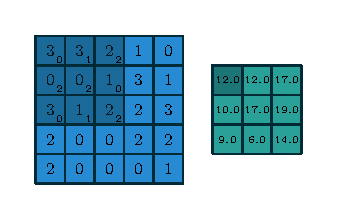
\includegraphics[width=0.3\textwidth]
        {pdf/numerical_no_padding_no_strides_00.pdf}
    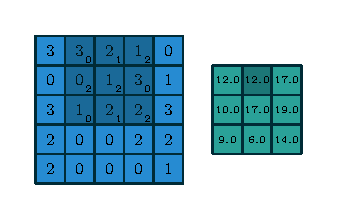
\includegraphics[width=0.3\textwidth]
        {pdf/numerical_no_padding_no_strides_01.pdf}
    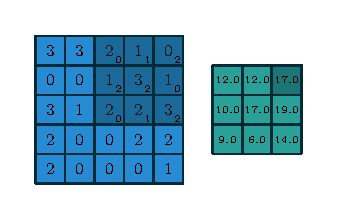
\includegraphics[width=0.3\textwidth]
        {pdf/numerical_no_padding_no_strides_02.pdf}
    \caption{\label{fig:numerical_no_padding_no_strides} Computing three output
        values of a discrete convolution.}
\end{figure}

If there are multiple input feature maps, each input feature map is convolved
with a distinct kernel, and the resulting feature maps are summed up elementwise
to produce the output feature map. The procedure can be repeated using different
kernels to form as many output feature maps as desired.

The convolution presented in \autoref{fig:numerical_no_padding_no_strides} is an
instance of a 2-D convolution, but it can be generalized to N-D convolutions.
For instance, in a 3-D convolution, the kernel would be a {\em cuboid} and would
slide across the height, width and depth of the input feature map.

The collection of kernels defining a discrete convolution has a shape
corresponding to some permutation of $(n, m, k_1, \ldots, k_N)$, where

\begin{equation}
\begin{split}
    n &\equiv \text{number of output feature maps},\\
    m &\equiv \text{number of input feature maps},\\
    k_j &\equiv \text{kernel size along axis $j$}.
\end{split}
\end{equation}

The following properties affect the output size $o_j$ of a convolutional layer
along axis $j$:

\begin{itemize}
    \item $i_j$: input size along axis $j$,
    \item $k_j$: kernel size along axis $j$,
    \item $s_j$: stride (distance between two consecutive positions of the
        kernel) along axis $j$,
    \item $p_j$: zero-padding (number of zeros concatenated at the beginning and
        at the end of an axis) along axis $j$.
\end{itemize}

For instance, \autoref{fig:numerical_padding_strides} shows a $3 \times 3$
kernel applied to a $5 \times 5$ input padded with a $1 \times 1$ border of
zeros using $2 \times 2$ strides.

\begin{figure}[t]
    \centering
    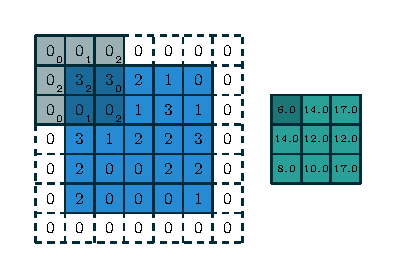
\includegraphics[width=0.3\textwidth]{pdf/numerical_padding_strides_00.pdf}
    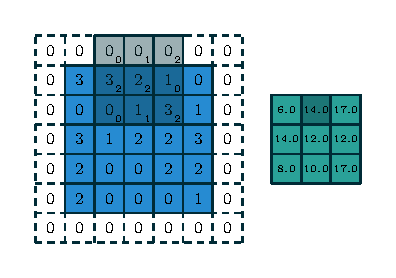
\includegraphics[width=0.3\textwidth]{pdf/numerical_padding_strides_01.pdf}
    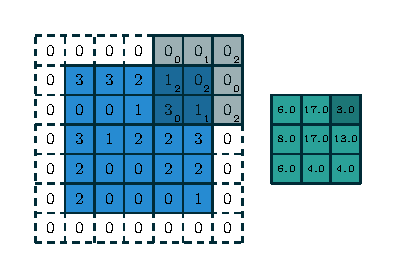
\includegraphics[width=0.3\textwidth]{pdf/numerical_padding_strides_02.pdf}
    \caption{\label{fig:numerical_padding_strides}Computing three output values
        of a discrete convolution for $N = 2$, $k_1 = k_2 = 3$, $s_1 = s_2 = 2$,
        and $p_1 = p_2 = 1$.}
\end{figure}

The analysis of the relationship between these parameters is simplified by the
fact that they don't interact across axes, i.e. choices of kernel size, stride
and zero padding along axis $i$ only affect the output size of axis $i$.

Because of this, the guide will concentrate on 2-D convolutional layers acting
on square inputs, and the kernel size, stride and zero-padding will always be
the same along both axes.

\bibliography{bibliography}
\bibliographystyle{natbib}
\end{document}
